\documentclass{memoria}
\usepackage[]{algorithm2e}


\begin{document}

\portada{Organización de Computadores: Laboratorio 1}{Nicolás Olivares}{Profesores:\\ Felipe Garay \\ Erika Rosas \\ Nicolás Hidalgo}{\today}


\indices

\capitulo{Introducción}
\seccion{Motivación}

\seccion{Objetivos}
\subseccion{Objetivo general}
El presente informe tiene como objetivo principal el análisis de un benchmark basado en MIPS en base a la aplicación de tareas de ordenamiento.
\subseccion{Objetivos específicos}
Dentro de los objetivos para este informe están:
\begin{enumerate}
\item Generar conjunto de programas, el cuál cuenta con dos programas de ordenamiento y uno de benchmark.
\item Fase de experimentación.
\item Análisis de los resultados.
\end{enumerate}
\seccion{Problema}
\emph{¿De qué manera se puede medir el rendimiento de un procesador?}\\Este informe presenta el planteamiento y solución a esta pregunta.
\seccion{Organización del documento}
El lector puede acceder a este documento y guiarse a través de los capítulos siguientes:
\begin{enumerate}
\item Introducción: la sección actual da al lector la información necesaria de preámbulo al tema  en cuestión, motivaciones y objetivos esperados.
\item Marco Teórico: en esta sección se hará un resumen explicativo de conceptos que el lector necesita entender en cierta medida para la mejor comprensión del fondo de este informe.
\item Desarrollo: en esta sección el lector podrá conocer en detalle el proceso de construcción de este laboratorio.
\item Análisis: el lector tendrá acceso a los razonamientos obtenidos a través de la realización  de experimentos sobre los programas construidos.
\item Para finalizar existe una sección de conclusiones para el informe, acerca del trabajo realizado y de la comparación entre objetivos y logros.
\end{enumerate}
\seccion{Herramientas}
Para la realización de este laboratorio se utilizaron las siguiente herramientas:
\begin{itemize}
\item Linux Mint 18 \emph{“Sarah”} \cite{mint}
\item Docker version 1.11.2, build b9f10c9 \cite{docker}
\item Sublime Text Build 3124 \cite{sublime}
\end{itemize}
\capitulo{Marco Teórico}
El lector debe entender este documento contiene términos técnicos que se explican en este capítulo, para expresarlos a manera de terminar en concenso para su lectura.
Sépase que la mención de instrucciones hace referencia a dos conceptos en este informe. Instrucciones estáticas corresponde a las instrucciones que un programador escribe en sus programas como líneas de código, llamense for, whiles u otros elementos que controlan el flujo del programa.Por otro lado las instrucciones dinámicas se establecen a nivel de máquina y procesador, como aquellas instrucciones que ejecuta el procesador y que dependen del conjunto de instrucciones en el cuál se trabaja.
\capitulo{Desarrollo}
\seccion{Preliminares}
Los programas se realizan en el lenguaje de programación C, con un paradigma de programación imperativo procedural.\\
Se utiliza docker engine para generar contenedores con la imagen y sistema de archivos proporcionado por el profesor Felipe Garay, de esta manera, dentro del container se tienen las herramientas de compilación necesarias como son mipsel-linux-gnu y sus diferentes opciones.
\seccion{Programas de ordenamiento}
Utilizando los conocimientos entregados en los cursos anteriores de la  carrera sobre el manejo de algoritmos, se implementaron dos algoritmos de ordenamiento de números enteros, \emph{ordenamiento de burbuja o bubblesort} y \emph{ordenamiento rapido o quicksort}.

\subseccion{Bubblesort}
El Algoritmo \ref{alg:bubble} corresponde al algoritmo de bubblesort, este algoritmo cuenta con una complejidad de instrucciones de orden O(n2).\cite{wiki:bubble}

\begin{algorithm}
\caption{Algoritmo bubblesort}\label{alg:bubble}
\SetKw{bubblesort}{bubblesort}
\KwData{Este algoritmo se encarga de ordenar un conjunto de números de menor a mayor.}
\KwIn{Conjunto A desordenado, n número de datos}
\KwOut{Conjunto A ordenado}
\bubblesort(A,n)
\For{$i=1$ to n}{
	\For{$j=n-i$ to 0}{
		\If{$A[j] > A[j+1]$}{
        	$aux = A[j]$\\
            $A[j]=A[j+1]$\\
            $A[j+1]=aux$
        }
	}
}
\end{algorithm}

\subseccion{Quicksort}
El Algoritmo \ref{alg:quick} corresponde a un algoritmo de caracter recursivo el cual presenta un orden de complejidad de instrucciones O(nlogn) para el caso promedio y O(n2) para el peor caso.\cite{quicksort_page}\cite{quicksort_video}

\begin{algorithm}
\caption{Algoritmo quicksort}\label{alg:quick}
\SetKw{quicksort}{quicksort}
\KwData{Este algoritmo se encarga de ordenar un conjunto de números de menor a mayor.}
\KwIn{Conjunto A desordenado, inicio, fin}
\KwOut{Conjunto A ordenado}
\quicksort($A,inicio,f$)
$i = inicio$\\
$f = fin$\\
$pivote = arreglo[(i+f)/2]$\\
\While{$i\leq f$}{
	\While{$A[i]<pivote$}{
		$i = i + 1$
	}
	\While{$A[f]>pivote$}{
		$f = f + 1$
	}
	\If{$i \leq f$}{$aux = A[i]$\\$A[i]=A[f]$\\A[f]=aux;\\$i = i + 1$\\$f = f - 1$}
	}
	\If{$inicio < f$}{\quicksort($A,inicio,f$)}
	\If{$fin > i$}{\quicksort($A,i,fin$)}
\end{algorithm}

Luego de tener ambos algoritmos e implementarlos se pasa a la fase de construcción del benchmark.
\seccion{Benchmark}
\subseccion{Requerimientos para la construcción del benchmark}
Con el uso de Docker Engine se utiliza un contenedor para cargar la imagen que el profesor Felipe Garay nos facilitó vía hub. Esta imagen corresponde a un sistema UFS o Unix File System, donde esta disponible una herramienta de emulación llamada qemu
\subseccion{Análisis previo}
Para el cálculo de MIPS se da la siguiente fórmula en el enunciado del laboratorio
\begin{equation}
\label{eqn:mips_preliminar}
MIPS = \frac{NI}{T \times 10^6}
\end{equation}
En la fórmula \ref{eqn:mips_preliminar}, NI representa el \emph{número de instrucciones} de un programa, mientras que T representa el \emph{Tiempo de ejecución} del programa.\cite{mips_formula}
Ahora bien, ¿Cómo obtener tanto NI y T para la fórmula dada?
En base al código C de los programas de ordenamiento, se obtienen, mediante decompilación las instrucciones del conjunto MIPS que son ejecutadas a nivel de procesador. Se contabilizan de estas instrucciones, separando aquellas que pertenecen al tipo I, tipo R y tipo J, 
\\
\subseccion{Abordando el problema}
\subsubseccion{Cálculo de MIPS}
En base al análisis previo realizado, se describen a continuación una serie de hechos y supuestos para el cálculo de MIPS en el programa de Benchmark.
\begin{itemize}
\item El cálculo de MIPS y tiempos de ejecución se realizan sólo para las instrucciones de la subrutina de ordenamiento, utilizando la librería {"sys/time.h"}.
\item Considerando que se trabaja con el set de instrucciones de MIPS, esto implica que existen 3 tipos de instrucciones, I, R, J.
\end{itemize}
Luego de la decompilación del programa, se contabilizan las instrucciones según su tipo. A continuación se presentan las proporciones obtenidas de la contabilización de las instrucciones.

\figura{Proporción de instrucciones dinámicas según su tipo para Algoritmo \ref{alg:bubble}}{\includegraphics[width = \textwidth]{Tabla_proporciones_iter.png}}{fig:tabla_prop_iter}

\figura{Proporción de instrucciones dinámicas según su tipo para Algoritmo \ref{alg:quick}}{\includegraphics[width = \textwidth]{Tabla_proporciones_rec.png}}{fig:tabla_prop_rec}

Para generar la \ref{fig:tabla_prop_iter} y la \ref{fig:tabla_prop_rec} se contabilizaron las instrucciones dinámicas de la subrutina de ordenamiento iterativa y recursiva. El objetivo de hacer esta identificación, es obtener las \emph{proporciones} de las instrucciones con respecto al total de instrucciones del algoritmo.

\figura{Porcentaje de intrucciones dinámicas afectado por las iteraciones en el Algoritmo \ref{alg:bubble}}{\includegraphics[width = \textwidth]{Tabla_porcentaje_Iterativo.png}}{fig:tabla_porc_iter}

\figura{Porcentaje de instrucciones dinámicas afectado por las recursiones en el Algoritmo \ref{alg:quick}}{\includegraphics[width = \textwidth]{Tabla_porcentaje_recursivo.png}}{fig:tabla_porc_rec}

En las tablas de las figuras \ref{fig:tabla_porc_rec} y \ref{fig:tabla_porc_iter}, se observa el reslutado de la lectura e interpretación de los archivos decompilados con las instrucciones de assembly MIPS. Esta interpretación representa una aproximación a que fracción de las instrucciones dínamicas del programa se ven afectadas o se ejecutan mas de una vez debido a que las instrucciones estáticas así lo demandan debido a loops, whiles u otros métodos de control involucrados en la programación de los programas.\cite{computer_organization}.
\\
Dicho todo esto, se procede a construir el programa de benchmark para obtener los Millones de Instrucciones Por Segundo mediante la ecuación \ref{eqn:mips_preliminar} y también los tiempos estimados de ejecución del programa, y especificamente, de la porción que realiza el ordenamiento.
\capitulo{Análisis}
Para este capítulo se declaran a continuación algunos hechos y supuestos que deben estar presentes durante el análisis.

\begin{itemize}
\item La máquina usada para las pruebas es un laptop personal, dentro de sus características están.
  \begin{itemize}
      \item Procesador: Intel(R) Core(TM) i5-2450M CPU @2.50GHz de cuatro núcleos de proceso.
      \item Memoria: 8GB RAM.
      \item Sistema Operativo: Linux Mint "Sarah".
      \item Dispositivos de entrada estandard para laptop.
	\end{itemize}
\item El cálculo aproximado de tiempos, representa una aproximación a las cantidades reales medibles de parámetros.
\item Para la prueba de los experimentos y su análisis, se utiliza una entrada de 20000 datos.
\end{itemize}

La figura \ref{fig:resultado_benchmark} muestra los resultados obtenidos del benchmark ejecutado en mi computador.

\figura{Datos de salida de Benchmark}{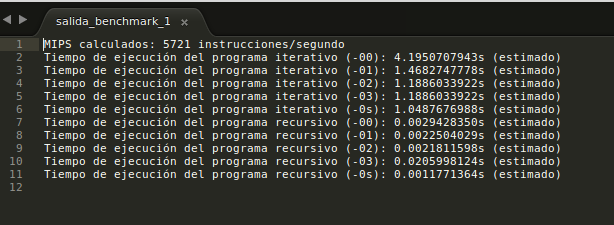
\includegraphics[width =\textwidth]{resultados.png}}{fig:resultado_benchmark}

\seccion{Experimentos}
Se definen los tres experimentos a realizar:
\begin{itemize}
\item \emph{EXP 01}: Medición de los tiempos reales de ejecución con time.h para bubblesort y quicksort, comparación con tiempo estimado de benchmark, con la máquina en el siguiente estado:
\begin{itemize}
\item Prendida por más de 16 hrs consecutivas.
\item Reproduciendo streaming de video y música.
\item Conectada a corriente eléctrica.
\end{itemize}
\item \emph{EXP 02}: Medición de los tiempos reales de ejecución con time.h para bubblesort y quicksort, comparación con tiempo estimado de benchmark, con la máquina en el siguiente estado:
\begin{itemize}
\item No más de 10 minutos desde su encendido, sin correr ningún programa o tarea extra además de los programas de inicio.
\item Conectada a corriente eléctrica.
\end{itemize}
\item \emph{EXP 03}: Medición de los tiempos reales de ejecución con time.h para bubblesort y quicksort, comparación con tiempo estimado de benchmark, con la máquina en el siguiente estado:
\begin{itemize}
\item No más de 10 minutos desde su encendido, sin correr ningún programa o tarea extra además de los programas de inicio.
\item Solo con suministro de batería.
\end{itemize}
\end{itemize}
\subseccion{Experimento No 1}
\subsubseccion{Hipótesis}
 \emph{Dada la acumulación de tareas en el procesador durante el tiempo en que la máquina permance encendida, sumado al uso de buffers y procesamiento para streaming, el valor de los tiempos de ejecución deberían estar a un nivel más bien cercano al estimado, con una diferencia de a lo más 0.5 segundos }
\subsubseccion{Resultados}
\figura{Resultados Experimento 01}{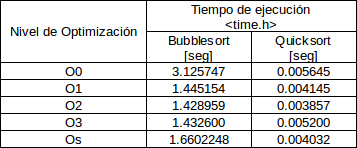
\includegraphics[width = \textwidth]{exp02.png}}{fig:exp1}
\subseccion{Experimento No 2}
\subsubseccion{Hipótesis}
\emph{Dado que al encender la máquina luego de un estado de apagado, las tareas ejecutadas en un inicio son las mínimas, el valor de los tiempos de ejecución deberá estar alejado del tiempo esperado en a lo más 1 segundo }
\subsubseccion{Resultados}
\figura{Resultados Experimento 02}{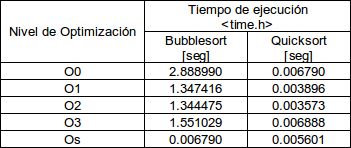
\includegraphics[width = \textwidth]{exp03.png}}{fig:exp2}
\subseccion{Experimento No 3}
\subsubseccion{Hipótesis}
\emph{Dado que al encender la máquina luego de un estado de apagado, las tareas ejecutadas en un inicio son las mínimas, y considerando que la máquina con batería entra en modo de eficiencia, el valor de los tiempos de ejecución deberá estar alejado del tiempo esperado en a lo más 1.2 segundos }
\subsubseccion{Resultados}
\figura{Resultados Experimento 03}{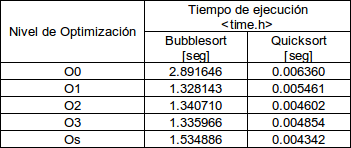
\includegraphics[width = \textwidth]{exp04.png}}{fig:exp3}
\section{Análisis de resultados}
\subsection{Con respecto a...}
\subsubseccion{Nivel de optimización}
Según  \ref{fig:exp1}, \ref{fig:exp2}, y \ref{fig:exp3}, se puede decir que el nivel O0 presenta un menor grado optimización con respecto a los demás niveles para el algoritmo de bubblesort, ya que de acuerdo a la decompilación aplicada, este nivel presentaba cerca de 74 instrucciones dinámicas que son cerca de 45 instrucciones más que los demás niveles de bubblesort que rondaban entre las 20 a 25 instrucciones,véase \ref{fig:tabla_prop_iter}.\\
Para el caso del algoritmo recursivo de quicksort, aquella optimización que entrega un menor grado de optimización y por consecuente un mayor número de intrucciones es el nivel O3; para este nivel en particular se generaron 620 instrucciones dinámicas en el decompilado, véase \ref{fig:tabla_prop_rec}.
Todo esto se debe a que los algoritmos fueron compilados con 5 niveles de optimización  distintos, según el compilador, esto generó más o menos instrucciones de MIPS según el nivel.
\subsubseccion{Tiempo real vs Tiempo estimado}
Por parte del algoritmo bubblesort, este se aproxima cercanamente al resultado del benchmark para la máquina, quedando unos más o menos entre 0.5 a 1 segundo por debajo o arriba del tiempo estimado. Así como también el algoritmo de quicksort donde el fallo de la estimación es de unos más o menos 0.003 segundos en cada nivel.
\subsubseccion{Experimentos}
Evaluando el desempeño de los niveles y algoritmos en relación a los resultados obtenidos nos lleva a las siguiente análisis:
\begin{enumerate}
\item En el caso del EXP01 existe evidencia para rechazar la hipótesis ya que el valor real obtenido difiere del estimado en 1.13 segundos en el caso del algoritmo de bubblesort. ¿A qué se debe esto?, por una parte es posible y probable que el cálculo del benchmark para los tiempos estimados dado los MIPS obtenidos, sea más abultado que la realidad, ya que el cálculo de los tiempos de ejecucion aproximados en base a las proporciones, no estan implementados correctamente. Pero se puede aceptar la hipótesis si se evalua el desempeño con los otros niveles de optimización, los cuales difieren del estimado en 0.3 segundos aproximadamente, como lo refleja la \ref{fig:exp1}.
\item En base a lo explicado para el experimento 1 y con la evidencia de la \ref{fig:exp2} se puede aceptar la hipótesis como verdadera, ya que ls valores reales comparados con la estimación presentan una variacón de menos de 1 segundo, descartando el nivel O0 dado bajo grado de optimización que posee.
Se destaca además que los tiempos del experimento son más bajos que los tiempos obtenidos en el experimento 1,\ref{fig:exp1}, ya que el procesador tenía una menor sobrecarga de tareas durante el momento de ejecución del experimento 2.
\item Pese a lo planteado en la hipótesis, en donde se esperaba que dado la falta de corriente eléctrica directa de la red, se produjera un ascenco en el tiempo real debido a gran parte de las máquinas actuales, tienen frcuencias de reloj variable, y que en momentos de \emph{sólo batería} presentan frecuencias más bajas por lo tanto una disminución en la capacidad de procesar más instrucciones por segundo. Los resultados en la \ref{fig:exp3} indican un rechazo a esta hipótesis. Aunque esto puede deberse a que la distribución de Linxu que se usó para la experimentación no maneje de manera eficiente el control de frecuencias del procesador.
\end{enumerate}

\capitulo{Conclusión}
Ya para finalizar este informe de análisis sobre el uso de la estrategia de benchmarking MIPS o Millions Instructions Per Second. A continuación se compara el estado previo al desarrollo de este documento, con los objetivos y logros.
\\Se presentan las comparaciones con los objetivos específicos planteados.
\begin{enumerate}
\item Se cumplió el objetivo de generar el conjunto de programas de pedidos; dos programas de ordenamiento fueron creados de manera exitosa, cumpliendo su objetivo final. Por otro lado el programa de benchmark cumple su función de referencia, pero algunos aspectos dentro del programa no representan una correcta implementación.
\item Se realizó una fase de experimentación, abordando aspectos de cómo la máquina
\end{enumerate}
\seccion{Respuesta a la interrogante}
Se planteó en el inicio una pregunta \emph{¿De qué manera se puede medir el rendimiento de un procesador?}


\bibliografiasincita
\end{document}
